%\documentclass{standalone}
%\usepackage{tikz}
%\usetikzlibrary{patterns,plotmarks}
%\begin{document}
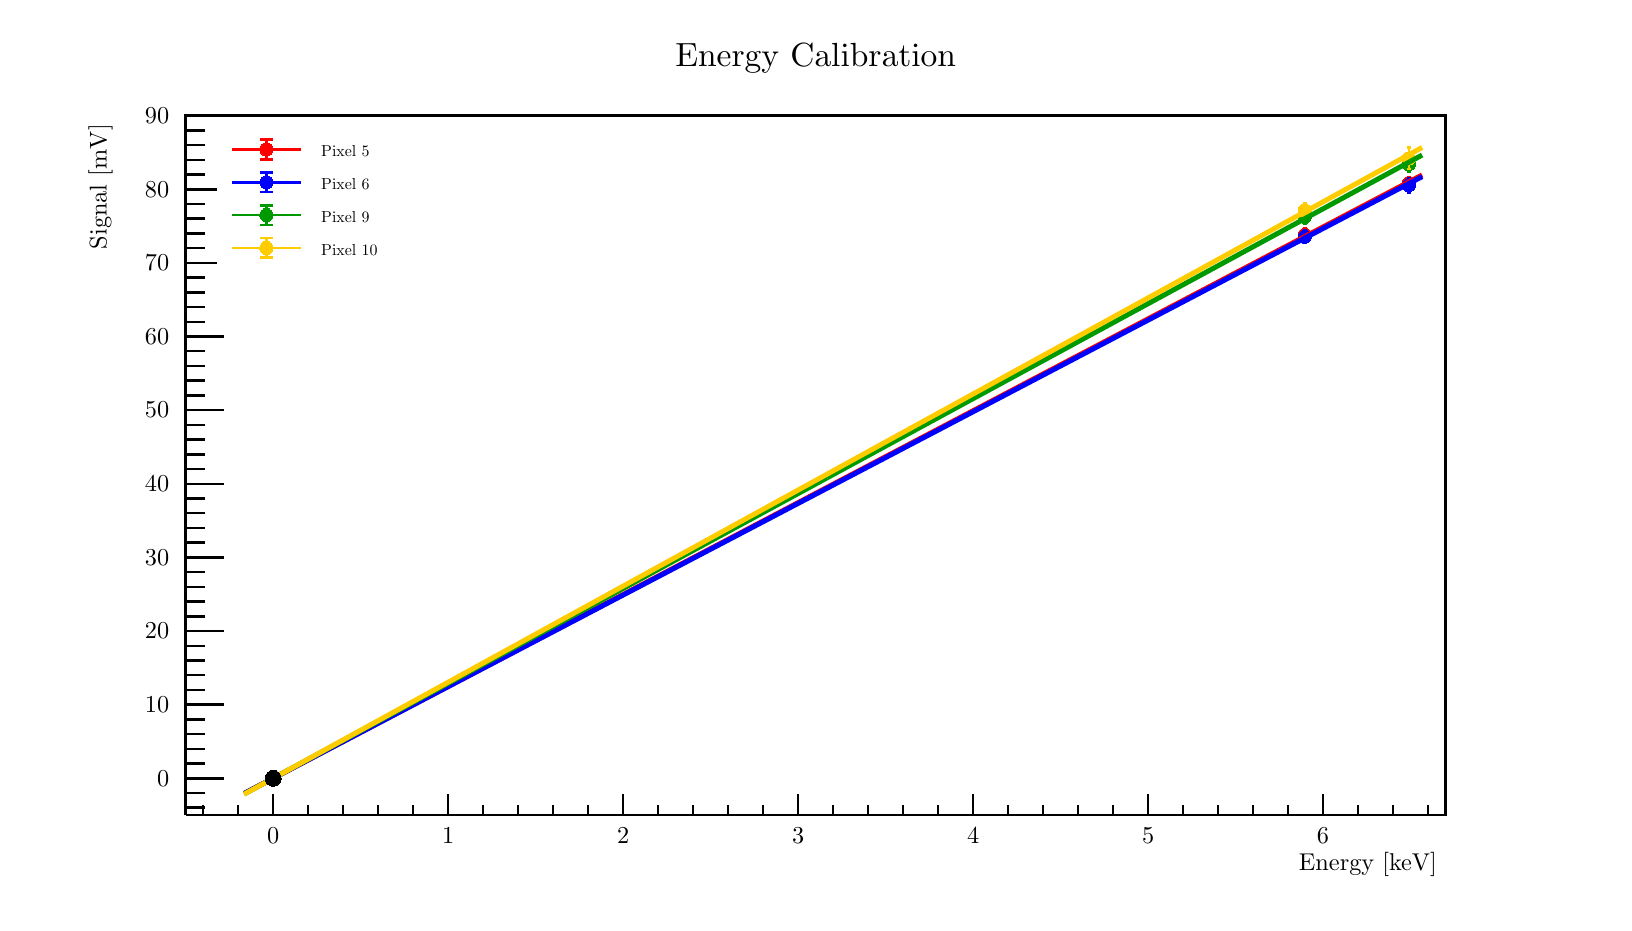
\begin{tikzpicture}
\def\CheckTikzLibraryLoaded#1{ \ifcsname tikz@library@#1@loaded\endcsname \else \PackageWarning{tikz}{usetikzlibrary{#1} is missing in the preamble.} \fi }
\CheckTikzLibraryLoaded{patterns}
\CheckTikzLibraryLoaded{plotmarks}
\pgfdeclareplotmark{cross} {
\pgfpathmoveto{\pgfpoint{-0.3\pgfplotmarksize}{\pgfplotmarksize}}
\pgfpathlineto{\pgfpoint{+0.3\pgfplotmarksize}{\pgfplotmarksize}}
\pgfpathlineto{\pgfpoint{+0.3\pgfplotmarksize}{0.3\pgfplotmarksize}}
\pgfpathlineto{\pgfpoint{+1\pgfplotmarksize}{0.3\pgfplotmarksize}}
\pgfpathlineto{\pgfpoint{+1\pgfplotmarksize}{-0.3\pgfplotmarksize}}
\pgfpathlineto{\pgfpoint{+0.3\pgfplotmarksize}{-0.3\pgfplotmarksize}}
\pgfpathlineto{\pgfpoint{+0.3\pgfplotmarksize}{-1.\pgfplotmarksize}}
\pgfpathlineto{\pgfpoint{-0.3\pgfplotmarksize}{-1.\pgfplotmarksize}}
\pgfpathlineto{\pgfpoint{-0.3\pgfplotmarksize}{-0.3\pgfplotmarksize}}
\pgfpathlineto{\pgfpoint{-1.\pgfplotmarksize}{-0.3\pgfplotmarksize}}
\pgfpathlineto{\pgfpoint{-1.\pgfplotmarksize}{0.3\pgfplotmarksize}}
\pgfpathlineto{\pgfpoint{-0.3\pgfplotmarksize}{0.3\pgfplotmarksize}}
\pgfpathclose
\pgfusepathqstroke
}
\pgfdeclareplotmark{cross*} {
\pgfpathmoveto{\pgfpoint{-0.3\pgfplotmarksize}{\pgfplotmarksize}}
\pgfpathlineto{\pgfpoint{+0.3\pgfplotmarksize}{\pgfplotmarksize}}
\pgfpathlineto{\pgfpoint{+0.3\pgfplotmarksize}{0.3\pgfplotmarksize}}
\pgfpathlineto{\pgfpoint{+1\pgfplotmarksize}{0.3\pgfplotmarksize}}
\pgfpathlineto{\pgfpoint{+1\pgfplotmarksize}{-0.3\pgfplotmarksize}}
\pgfpathlineto{\pgfpoint{+0.3\pgfplotmarksize}{-0.3\pgfplotmarksize}}
\pgfpathlineto{\pgfpoint{+0.3\pgfplotmarksize}{-1.\pgfplotmarksize}}
\pgfpathlineto{\pgfpoint{-0.3\pgfplotmarksize}{-1.\pgfplotmarksize}}
\pgfpathlineto{\pgfpoint{-0.3\pgfplotmarksize}{-0.3\pgfplotmarksize}}
\pgfpathlineto{\pgfpoint{-1.\pgfplotmarksize}{-0.3\pgfplotmarksize}}
\pgfpathlineto{\pgfpoint{-1.\pgfplotmarksize}{0.3\pgfplotmarksize}}
\pgfpathlineto{\pgfpoint{-0.3\pgfplotmarksize}{0.3\pgfplotmarksize}}
\pgfpathclose
\pgfusepathqfillstroke
}
\pgfdeclareplotmark{newstar} {
\pgfpathmoveto{\pgfqpoint{0pt}{\pgfplotmarksize}}
\pgfpathlineto{\pgfqpointpolar{44}{0.5\pgfplotmarksize}}
\pgfpathlineto{\pgfqpointpolar{18}{\pgfplotmarksize}}
\pgfpathlineto{\pgfqpointpolar{-20}{0.5\pgfplotmarksize}}
\pgfpathlineto{\pgfqpointpolar{-54}{\pgfplotmarksize}}
\pgfpathlineto{\pgfqpointpolar{-90}{0.5\pgfplotmarksize}}
\pgfpathlineto{\pgfqpointpolar{234}{\pgfplotmarksize}}
\pgfpathlineto{\pgfqpointpolar{198}{0.5\pgfplotmarksize}}
\pgfpathlineto{\pgfqpointpolar{162}{\pgfplotmarksize}}
\pgfpathlineto{\pgfqpointpolar{134}{0.5\pgfplotmarksize}}
\pgfpathclose
\pgfusepathqstroke
}
\pgfdeclareplotmark{newstar*} {
\pgfpathmoveto{\pgfqpoint{0pt}{\pgfplotmarksize}}
\pgfpathlineto{\pgfqpointpolar{44}{0.5\pgfplotmarksize}}
\pgfpathlineto{\pgfqpointpolar{18}{\pgfplotmarksize}}
\pgfpathlineto{\pgfqpointpolar{-20}{0.5\pgfplotmarksize}}
\pgfpathlineto{\pgfqpointpolar{-54}{\pgfplotmarksize}}
\pgfpathlineto{\pgfqpointpolar{-90}{0.5\pgfplotmarksize}}
\pgfpathlineto{\pgfqpointpolar{234}{\pgfplotmarksize}}
\pgfpathlineto{\pgfqpointpolar{198}{0.5\pgfplotmarksize}}
\pgfpathlineto{\pgfqpointpolar{162}{\pgfplotmarksize}}
\pgfpathlineto{\pgfqpointpolar{134}{0.5\pgfplotmarksize}}
\pgfpathclose
\pgfusepathqfillstroke
}
\definecolor{c}{rgb}{1,1,1};
\draw [color=c, fill=c] (0,0) rectangle (20,11.1035);
\draw [color=c, fill=c] (2,1.11035) rectangle (18,9.99319);
\definecolor{c}{rgb}{0,0,0};
\draw [c,line width=0.9] (2,1.11035) -- (2,9.99319) -- (18,9.99319) -- (18,1.11035) -- (2,1.11035);
\definecolor{c}{rgb}{1,1,1};
\draw [color=c, fill=c] (2,1.11035) rectangle (18,9.99319);
\definecolor{c}{rgb}{0,0,0};
\draw [c,line width=0.9] (2,1.11035) -- (2,9.99319) -- (18,9.99319) -- (18,1.11035) -- (2,1.11035);
\draw [c,line width=0.9] (2,1.11035) -- (18,1.11035);
\draw [c,line width=0.9] (3.11111,1.37684) -- (3.11111,1.11035);
\draw [c,line width=0.9] (3.55556,1.2436) -- (3.55556,1.11035);
\draw [c,line width=0.9] (4,1.2436) -- (4,1.11035);
\draw [c,line width=0.9] (4.44444,1.2436) -- (4.44444,1.11035);
\draw [c,line width=0.9] (4.88889,1.2436) -- (4.88889,1.11035);
\draw [c,line width=0.9] (5.33333,1.37684) -- (5.33333,1.11035);
\draw [c,line width=0.9] (5.77778,1.2436) -- (5.77778,1.11035);
\draw [c,line width=0.9] (6.22222,1.2436) -- (6.22222,1.11035);
\draw [c,line width=0.9] (6.66667,1.2436) -- (6.66667,1.11035);
\draw [c,line width=0.9] (7.11111,1.2436) -- (7.11111,1.11035);
\draw [c,line width=0.9] (7.55556,1.37684) -- (7.55556,1.11035);
\draw [c,line width=0.9] (8,1.2436) -- (8,1.11035);
\draw [c,line width=0.9] (8.44444,1.2436) -- (8.44444,1.11035);
\draw [c,line width=0.9] (8.88889,1.2436) -- (8.88889,1.11035);
\draw [c,line width=0.9] (9.33333,1.2436) -- (9.33333,1.11035);
\draw [c,line width=0.9] (9.77778,1.37684) -- (9.77778,1.11035);
\draw [c,line width=0.9] (10.2222,1.2436) -- (10.2222,1.11035);
\draw [c,line width=0.9] (10.6667,1.2436) -- (10.6667,1.11035);
\draw [c,line width=0.9] (11.1111,1.2436) -- (11.1111,1.11035);
\draw [c,line width=0.9] (11.5556,1.2436) -- (11.5556,1.11035);
\draw [c,line width=0.9] (12,1.37684) -- (12,1.11035);
\draw [c,line width=0.9] (12.4444,1.2436) -- (12.4444,1.11035);
\draw [c,line width=0.9] (12.8889,1.2436) -- (12.8889,1.11035);
\draw [c,line width=0.9] (13.3333,1.2436) -- (13.3333,1.11035);
\draw [c,line width=0.9] (13.7778,1.2436) -- (13.7778,1.11035);
\draw [c,line width=0.9] (14.2222,1.37684) -- (14.2222,1.11035);
\draw [c,line width=0.9] (14.6667,1.2436) -- (14.6667,1.11035);
\draw [c,line width=0.9] (15.1111,1.2436) -- (15.1111,1.11035);
\draw [c,line width=0.9] (15.5556,1.2436) -- (15.5556,1.11035);
\draw [c,line width=0.9] (16,1.2436) -- (16,1.11035);
\draw [c,line width=0.9] (16.4444,1.37684) -- (16.4444,1.11035);
\draw [c,line width=0.9] (2.66667,1.2436) -- (2.66667,1.11035);
\draw [c,line width=0.9] (2.22222,1.2436) -- (2.22222,1.11035);
\draw [c,line width=0.9] (16.8889,1.2436) -- (16.8889,1.11035);
\draw [c,line width=0.9] (17.3333,1.2436) -- (17.3333,1.11035);
\draw [c,line width=0.9] (17.7778,1.2436) -- (17.7778,1.11035);
\draw [anchor=base] (3.11111,0.743937) node[scale=0.877495, color=c, rotate=0]{0};
\draw [anchor=base] (5.33333,0.743937) node[scale=0.877495, color=c, rotate=0]{1};
\draw [anchor=base] (7.55556,0.743937) node[scale=0.877495, color=c, rotate=0]{2};
\draw [anchor=base] (9.77778,0.743937) node[scale=0.877495, color=c, rotate=0]{3};
\draw [anchor=base] (12,0.743937) node[scale=0.877495, color=c, rotate=0]{4};
\draw [anchor=base] (14.2222,0.743937) node[scale=0.877495, color=c, rotate=0]{5};
\draw [anchor=base] (16.4444,0.743937) node[scale=0.877495, color=c, rotate=0]{6};
\draw [anchor= east] (18,0.488556) node[scale=0.877495, color=c, rotate=0]{Energy [keV]};
\draw [c,line width=0.9] (2,1.11035) -- (2,9.99319);
\draw [c,line width=0.9] (2.48,1.57787) -- (2,1.57787);
\draw [c,line width=0.9] (2.24,1.76488) -- (2,1.76488);
\draw [c,line width=0.9] (2.24,1.95189) -- (2,1.95189);
\draw [c,line width=0.9] (2.24,2.13889) -- (2,2.13889);
\draw [c,line width=0.9] (2.24,2.3259) -- (2,2.3259);
\draw [c,line width=0.9] (2.48,2.51291) -- (2,2.51291);
\draw [c,line width=0.9] (2.24,2.69991) -- (2,2.69991);
\draw [c,line width=0.9] (2.24,2.88692) -- (2,2.88692);
\draw [c,line width=0.9] (2.24,3.07393) -- (2,3.07393);
\draw [c,line width=0.9] (2.24,3.26094) -- (2,3.26094);
\draw [c,line width=0.9] (2.48,3.44794) -- (2,3.44794);
\draw [c,line width=0.9] (2.24,3.63495) -- (2,3.63495);
\draw [c,line width=0.9] (2.24,3.82196) -- (2,3.82196);
\draw [c,line width=0.9] (2.24,4.00896) -- (2,4.00896);
\draw [c,line width=0.9] (2.24,4.19597) -- (2,4.19597);
\draw [c,line width=0.9] (2.48,4.38298) -- (2,4.38298);
\draw [c,line width=0.9] (2.24,4.56998) -- (2,4.56998);
\draw [c,line width=0.9] (2.24,4.75699) -- (2,4.75699);
\draw [c,line width=0.9] (2.24,4.944) -- (2,4.944);
\draw [c,line width=0.9] (2.24,5.13101) -- (2,5.13101);
\draw [c,line width=0.9] (2.48,5.31801) -- (2,5.31801);
\draw [c,line width=0.9] (2.24,5.50502) -- (2,5.50502);
\draw [c,line width=0.9] (2.24,5.69203) -- (2,5.69203);
\draw [c,line width=0.9] (2.24,5.87903) -- (2,5.87903);
\draw [c,line width=0.9] (2.24,6.06604) -- (2,6.06604);
\draw [c,line width=0.9] (2.48,6.25305) -- (2,6.25305);
\draw [c,line width=0.9] (2.24,6.44005) -- (2,6.44005);
\draw [c,line width=0.9] (2.24,6.62706) -- (2,6.62706);
\draw [c,line width=0.9] (2.24,6.81407) -- (2,6.81407);
\draw [c,line width=0.9] (2.24,7.00108) -- (2,7.00108);
\draw [c,line width=0.9] (2.48,7.18808) -- (2,7.18808);
\draw [c,line width=0.9] (2.24,7.37509) -- (2,7.37509);
\draw [c,line width=0.9] (2.24,7.5621) -- (2,7.5621);
\draw [c,line width=0.9] (2.24,7.7491) -- (2,7.7491);
\draw [c,line width=0.9] (2.24,7.93611) -- (2,7.93611);
\draw [c,line width=0.9] (2.48,8.12312) -- (2,8.12312);
\draw [c,line width=0.9] (2.24,8.31012) -- (2,8.31012);
\draw [c,line width=0.9] (2.24,8.49713) -- (2,8.49713);
\draw [c,line width=0.9] (2.24,8.68414) -- (2,8.68414);
\draw [c,line width=0.9] (2.24,8.87115) -- (2,8.87115);
\draw [c,line width=0.9] (2.48,9.05815) -- (2,9.05815);
\draw [c,line width=0.9] (2.24,9.24516) -- (2,9.24516);
\draw [c,line width=0.9] (2.24,9.43217) -- (2,9.43217);
\draw [c,line width=0.9] (2.24,9.61917) -- (2,9.61917);
\draw [c,line width=0.9] (2.24,9.80618) -- (2,9.80618);
\draw [c,line width=0.9] (2.48,9.99319) -- (2,9.99319);
\draw [c,line width=0.9] (2.24,1.39086) -- (2,1.39086);
\draw [c,line width=0.9] (2.24,1.20386) -- (2,1.20386);
\draw [anchor= east] (1.9,1.57787) node[scale=0.877495, color=c, rotate=0]{0};
\draw [anchor= east] (1.9,2.51291) node[scale=0.877495, color=c, rotate=0]{10};
\draw [anchor= east] (1.9,3.44794) node[scale=0.877495, color=c, rotate=0]{20};
\draw [anchor= east] (1.9,4.38298) node[scale=0.877495, color=c, rotate=0]{30};
\draw [anchor= east] (1.9,5.31801) node[scale=0.877495, color=c, rotate=0]{40};
\draw [anchor= east] (1.9,6.25305) node[scale=0.877495, color=c, rotate=0]{50};
\draw [anchor= east] (1.9,7.18808) node[scale=0.877495, color=c, rotate=0]{60};
\draw [anchor= east] (1.9,8.12312) node[scale=0.877495, color=c, rotate=0]{70};
\draw [anchor= east] (1.9,9.05815) node[scale=0.877495, color=c, rotate=0]{80};
\draw [anchor= east] (1.9,9.99319) node[scale=0.877495, color=c, rotate=0]{90};
\draw [anchor= east] (0.918529,9.99319) node[scale=0.877495, color=c, rotate=90]{Signal [mV]};
\definecolor{c}{rgb}{1,0,0};
\draw [c,line width=0.9] (16.2111,8.53485) -- (16.2111,8.56217);
\draw [c,line width=0.9] (16.2111,8.42586) -- (16.2111,8.39855);
\draw [c,line width=0.9] (16.1839,8.56217) -- (16.2384,8.56217);
\draw [c,line width=0.9] (16.1839,8.39855) -- (16.2384,8.39855);
\draw [c,line width=0.9] (17.5333,9.18924) -- (17.5333,9.20697);
\draw [c,line width=0.9] (17.5333,9.08025) -- (17.5333,9.06252);
\draw [c,line width=0.9] (17.5061,9.20697) -- (17.5606,9.20697);
\draw [c,line width=0.9] (17.5061,9.06252) -- (17.5606,9.06252);
\foreach \P in {(16.2111,8.48036), (17.5333,9.13475)}{\draw[mark options={color=c,fill=c},mark size=2.402402pt, line width=0.000000pt, mark=*] plot coordinates {\P};}
\definecolor{c}{rgb}{0,0,1};
\draw [c,line width=0.9] (16.2111,8.51026) -- (16.2111,8.53878);
\draw [c,line width=0.9] (16.2111,8.40127) -- (16.2111,8.37275);
\draw [c,line width=0.9] (16.1839,8.53878) -- (16.2384,8.53878);
\draw [c,line width=0.9] (16.1839,8.37275) -- (16.2384,8.37275);
\draw [c,line width=0.9] (17.5333,9.16344) -- (17.5333,9.20333);
\draw [c,line width=0.9] (17.5333,9.05445) -- (17.5333,9.01455);
\draw [c,line width=0.9] (17.5061,9.20333) -- (17.5606,9.20333);
\draw [c,line width=0.9] (17.5061,9.01455) -- (17.5606,9.01455);
\foreach \P in {(16.2111,8.45577), (17.5333,9.10894)}{\draw[mark options={color=c,fill=c},mark size=2.402402pt, line width=0.000000pt, mark=*] plot coordinates {\P};}
\definecolor{c}{rgb}{0,0.6,0};
\draw [c,line width=0.9] (16.2111,8.7621) -- (16.2111,8.79577);
\draw [c,line width=0.9] (16.2111,8.65311) -- (16.2111,8.61944);
\draw [c,line width=0.9] (16.1839,8.79577) -- (16.2384,8.79577);
\draw [c,line width=0.9] (16.1839,8.61944) -- (16.2384,8.61944);
\draw [c,line width=0.9] (17.5333,9.43139) -- (17.5333,9.47052);
\draw [c,line width=0.9] (17.5333,9.3224) -- (17.5333,9.28326);
\draw [c,line width=0.9] (17.5061,9.47052) -- (17.5606,9.47052);
\draw [c,line width=0.9] (17.5061,9.28326) -- (17.5606,9.28326);
\foreach \P in {(16.2111,8.70761), (17.5333,9.37689)}{\draw[mark options={color=c,fill=c},mark size=2.402402pt, line width=0.000000pt, mark=*] plot coordinates {\P};}
\definecolor{c}{rgb}{1,0.8,0};
\draw [c,line width=0.9] (16.2111,8.84691) -- (16.2111,8.88182);
\draw [c,line width=0.9] (16.2111,8.73792) -- (16.2111,8.70302);
\draw [c,line width=0.9] (16.1839,8.88182) -- (16.2384,8.88182);
\draw [c,line width=0.9] (16.1839,8.70302) -- (16.2384,8.70302);
\draw [c,line width=0.9] (17.5333,9.50604) -- (17.5333,9.58671);
\draw [c,line width=0.9] (17.5333,9.39705) -- (17.5333,9.31638);
\draw [c,line width=0.9] (17.5061,9.58671) -- (17.5606,9.58671);
\draw [c,line width=0.9] (17.5061,9.31638) -- (17.5606,9.31638);
\foreach \P in {(16.2111,8.79242), (17.5333,9.45154)}{\draw[mark options={color=c,fill=c},mark size=2.402402pt, line width=0.000000pt, mark=*] plot coordinates {\P};}
\definecolor{c}{rgb}{1,1,1};
\draw [color=c, fill=c] (2.4,8.10559) rectangle (7.4,9.77112);
\definecolor{c}{rgb}{0,0,0};
\draw [anchor=base west] (3.65,9.46924) node[scale=0.57491, color=c, rotate=0]{Pixel 5};
\definecolor{c}{rgb}{1,0,0};
\draw [c,line width=0.9] (2.5875,9.56293) -- (3.4625,9.56293);
\draw [c,line width=0.9] (3.025,9.61742) -- (3.025,9.68784);
\draw [c,line width=0.9] (3.025,9.50843) -- (3.025,9.43801);
\draw [c,line width=0.9] (2.9375,9.68784) -- (3.1125,9.68784);
\draw [c,line width=0.9] (2.9375,9.43801) -- (3.1125,9.43801);
\foreach \P in {(3.025,9.56293)}{\draw[mark options={color=c,fill=c},mark size=2.402402pt, line width=0.000000pt, mark=*] plot coordinates {\P};}
\definecolor{c}{rgb}{0,0,0};
\draw [anchor=base west] (3.65,9.05286) node[scale=0.57491, color=c, rotate=0]{Pixel 6};
\definecolor{c}{rgb}{0,0,1};
\draw [c,line width=0.9] (2.5875,9.14654) -- (3.4625,9.14654);
\draw [c,line width=0.9] (3.025,9.20104) -- (3.025,9.27146);
\draw [c,line width=0.9] (3.025,9.09205) -- (3.025,9.02163);
\draw [c,line width=0.9] (2.9375,9.27146) -- (3.1125,9.27146);
\draw [c,line width=0.9] (2.9375,9.02163) -- (3.1125,9.02163);
\foreach \P in {(3.025,9.14654)}{\draw[mark options={color=c,fill=c},mark size=2.402402pt, line width=0.000000pt, mark=*] plot coordinates {\P};}
\definecolor{c}{rgb}{0,0,0};
\draw [anchor=base west] (3.65,8.63647) node[scale=0.57491, color=c, rotate=0]{Pixel 9};
\definecolor{c}{rgb}{0,0.6,0};
\draw [c,line width=0.9] (2.5875,8.73016) -- (3.4625,8.73016);
\draw [c,line width=0.9] (3.025,8.78466) -- (3.025,8.85507);
\draw [c,line width=0.9] (3.025,8.67566) -- (3.025,8.60525);
\draw [c,line width=0.9] (2.9375,8.85507) -- (3.1125,8.85507);
\draw [c,line width=0.9] (2.9375,8.60525) -- (3.1125,8.60525);
\foreach \P in {(3.025,8.73016)}{\draw[mark options={color=c,fill=c},mark size=2.402402pt, line width=0.000000pt, mark=*] plot coordinates {\P};}
\definecolor{c}{rgb}{0,0,0};
\draw [anchor=base west] (3.65,8.22009) node[scale=0.57491, color=c, rotate=0]{Pixel 10};
\definecolor{c}{rgb}{1,0.8,0};
\draw [c,line width=0.9] (2.5875,8.31378) -- (3.4625,8.31378);
\draw [c,line width=0.9] (3.025,8.36827) -- (3.025,8.43869);
\draw [c,line width=0.9] (3.025,8.25928) -- (3.025,8.18886);
\draw [c,line width=0.9] (2.9375,8.43869) -- (3.1125,8.43869);
\draw [c,line width=0.9] (2.9375,8.18886) -- (3.1125,8.18886);
\foreach \P in {(3.025,8.31378)}{\draw[mark options={color=c,fill=c},mark size=2.402402pt, line width=0.000000pt, mark=*] plot coordinates {\P};}
\definecolor{c}{rgb}{0,0,0};
\draw (10,10.7292) node[scale=1.21034, color=c, rotate=0]{Energy Calibration};
\definecolor{c}{rgb}{1,0,0};
\draw [c,line width=1.8] (2.74222,1.38416) -- (2.89333,1.46351) -- (3.04444,1.54286) -- (3.19556,1.62222) -- (3.34667,1.70157) -- (3.49778,1.78092) -- (3.64889,1.86027) -- (3.8,1.93962) -- (3.95111,2.01897) -- (4.10222,2.09833) -- (4.25333,2.17768)
 -- (4.40444,2.25703) -- (4.55556,2.33638) -- (4.70667,2.41573) -- (4.85778,2.49509) -- (5.00889,2.57444) -- (5.16,2.65379) -- (5.31111,2.73314) -- (5.46222,2.81249) -- (5.61333,2.89184) -- (5.76444,2.9712) -- (5.91556,3.05055) -- (6.06667,3.1299) --
 (6.21778,3.20925) -- (6.36889,3.2886) -- (6.52,3.36795) -- (6.67111,3.44731) -- (6.82222,3.52666) -- (6.97333,3.60601) -- (7.12444,3.68536) -- (7.27556,3.76471) -- (7.42667,3.84407) -- (7.57778,3.92342) -- (7.72889,4.00277) -- (7.88,4.08212) --
 (8.03111,4.16147) -- (8.18222,4.24082) -- (8.33333,4.32018) -- (8.48444,4.39953) -- (8.63556,4.47888) -- (8.78667,4.55823) -- (8.93778,4.63758) -- (9.08889,4.71694) -- (9.24,4.79629) -- (9.39111,4.87564) -- (9.54222,4.95499) -- (9.69333,5.03434) --
 (9.84444,5.11369) -- (9.99556,5.19305) -- (10.1467,5.2724);
\draw [c,line width=1.8] (10.1467,5.2724) -- (10.2978,5.35175) -- (10.4489,5.4311) -- (10.6,5.51045) -- (10.7511,5.5898) -- (10.9022,5.66916) -- (11.0533,5.74851) -- (11.2044,5.82786) -- (11.3556,5.90721) -- (11.5067,5.98656) -- (11.6578,6.06592) --
 (11.8089,6.14527) -- (11.96,6.22462) -- (12.1111,6.30397) -- (12.2622,6.38332) -- (12.4133,6.46267) -- (12.5644,6.54203) -- (12.7156,6.62138) -- (12.8667,6.70073) -- (13.0178,6.78008) -- (13.1689,6.85943) -- (13.32,6.93879) -- (13.4711,7.01814) --
 (13.6222,7.09749) -- (13.7733,7.17684) -- (13.9244,7.25619) -- (14.0756,7.33554) -- (14.2267,7.4149) -- (14.3778,7.49425) -- (14.5289,7.5736) -- (14.68,7.65295) -- (14.8311,7.7323) -- (14.9822,7.81165) -- (15.1333,7.89101) -- (15.2844,7.97036) --
 (15.4356,8.04971) -- (15.5867,8.12906) -- (15.7378,8.20841) -- (15.8889,8.28777) -- (16.04,8.36712) -- (16.1911,8.44647) -- (16.3422,8.52582) -- (16.4933,8.60517) -- (16.6444,8.68452) -- (16.7956,8.76388) -- (16.9467,8.84323) -- (17.0978,8.92258) --
 (17.2489,9.00193) -- (17.4,9.08128) -- (17.5511,9.16063);
\draw [c,line width=1.8] (17.5511,9.16063) -- (17.7022,9.23999);
\definecolor{c}{rgb}{0,0,1};
\draw [c,line width=1.8] (2.74222,1.3847) -- (2.89333,1.46383) -- (3.04444,1.54296) -- (3.19556,1.62209) -- (3.34667,1.70122) -- (3.49778,1.78035) -- (3.64889,1.85948) -- (3.8,1.93861) -- (3.95111,2.01774) -- (4.10222,2.09687) -- (4.25333,2.176) --
 (4.40444,2.25513) -- (4.55556,2.33426) -- (4.70667,2.41339) -- (4.85778,2.49252) -- (5.00889,2.57165) -- (5.16,2.65078) -- (5.31111,2.72991) -- (5.46222,2.80904) -- (5.61333,2.88817) -- (5.76444,2.9673) -- (5.91556,3.04643) -- (6.06667,3.12556) --
 (6.21778,3.20469) -- (6.36889,3.28382) -- (6.52,3.36295) -- (6.67111,3.44208) -- (6.82222,3.52121) -- (6.97333,3.60034) -- (7.12444,3.67947) -- (7.27556,3.7586) -- (7.42667,3.83773) -- (7.57778,3.91686) -- (7.72889,3.99599) -- (7.88,4.07512) --
 (8.03111,4.15425) -- (8.18222,4.23338) -- (8.33333,4.31251) -- (8.48444,4.39164) -- (8.63556,4.47077) -- (8.78667,4.5499) -- (8.93778,4.62903) -- (9.08889,4.70816) -- (9.24,4.78729) -- (9.39111,4.86642) -- (9.54222,4.94555) -- (9.69333,5.02468) --
 (9.84444,5.10381) -- (9.99556,5.18294) -- (10.1467,5.26207);
\draw [c,line width=1.8] (10.1467,5.26207) -- (10.2978,5.3412) -- (10.4489,5.42033) -- (10.6,5.49945) -- (10.7511,5.57859) -- (10.9022,5.65771) -- (11.0533,5.73685) -- (11.2044,5.81597) -- (11.3556,5.8951) -- (11.5067,5.97423) -- (11.6578,6.05336) --
 (11.8089,6.13249) -- (11.96,6.21162) -- (12.1111,6.29075) -- (12.2622,6.36988) -- (12.4133,6.44901) -- (12.5644,6.52814) -- (12.7156,6.60727) -- (12.8667,6.6864) -- (13.0178,6.76553) -- (13.1689,6.84466) -- (13.32,6.92379) -- (13.4711,7.00292) --
 (13.6222,7.08205) -- (13.7733,7.16118) -- (13.9244,7.24031) -- (14.0756,7.31944) -- (14.2267,7.39857) -- (14.3778,7.4777) -- (14.5289,7.55683) -- (14.68,7.63596) -- (14.8311,7.71509) -- (14.9822,7.79422) -- (15.1333,7.87335) -- (15.2844,7.95248) --
 (15.4356,8.03161) -- (15.5867,8.11074) -- (15.7378,8.18987) -- (15.8889,8.269) -- (16.04,8.34813) -- (16.1911,8.42726) -- (16.3422,8.50639) -- (16.4933,8.58552) -- (16.6444,8.66465) -- (16.7956,8.74378) -- (16.9467,8.82291) -- (17.0978,8.90204) --
 (17.2489,8.98117) -- (17.4,9.0603) -- (17.5511,9.13943);
\draw [c,line width=1.8] (17.5511,9.13943) -- (17.7022,9.21856);
\definecolor{c}{rgb}{0,0.6,0};
\draw [c,line width=1.8] (2.74222,1.37777) -- (2.89333,1.45974) -- (3.04444,1.54171) -- (3.19556,1.62368) -- (3.34667,1.70565) -- (3.49778,1.78762) -- (3.64889,1.86959) -- (3.8,1.95156) -- (3.95111,2.03353) -- (4.10222,2.1155) -- (4.25333,2.19747) --
 (4.40444,2.27944) -- (4.55556,2.36141) -- (4.70667,2.44338) -- (4.85778,2.52535) -- (5.00889,2.60731) -- (5.16,2.68928) -- (5.31111,2.77125) -- (5.46222,2.85322) -- (5.61333,2.93519) -- (5.76444,3.01716) -- (5.91556,3.09913) -- (6.06667,3.1811) --
 (6.21778,3.26307) -- (6.36889,3.34504) -- (6.52,3.42701) -- (6.67111,3.50898) -- (6.82222,3.59095) -- (6.97333,3.67292) -- (7.12444,3.75489) -- (7.27556,3.83686) -- (7.42667,3.91883) -- (7.57778,4.0008) -- (7.72889,4.08277) -- (7.88,4.16474) --
 (8.03111,4.24671) -- (8.18222,4.32868) -- (8.33333,4.41065) -- (8.48444,4.49262) -- (8.63556,4.57459) -- (8.78667,4.65656) -- (8.93778,4.73853) -- (9.08889,4.8205) -- (9.24,4.90247) -- (9.39111,4.98444) -- (9.54222,5.06641) -- (9.69333,5.14838) --
 (9.84444,5.23035) -- (9.99556,5.31231) -- (10.1467,5.39428);
\draw [c,line width=1.8] (10.1467,5.39428) -- (10.2978,5.47625) -- (10.4489,5.55822) -- (10.6,5.64019) -- (10.7511,5.72216) -- (10.9022,5.80413) -- (11.0533,5.8861) -- (11.2044,5.96807) -- (11.3556,6.05004) -- (11.5067,6.13201) -- (11.6578,6.21398)
 -- (11.8089,6.29595) -- (11.96,6.37792) -- (12.1111,6.45989) -- (12.2622,6.54186) -- (12.4133,6.62383) -- (12.5644,6.7058) -- (12.7156,6.78777) -- (12.8667,6.86974) -- (13.0178,6.95171) -- (13.1689,7.03368) -- (13.32,7.11565) -- (13.4711,7.19762) --
 (13.6222,7.27959) -- (13.7733,7.36156) -- (13.9244,7.44353) -- (14.0756,7.5255) -- (14.2267,7.60747) -- (14.3778,7.68944) -- (14.5289,7.77141) -- (14.68,7.85338) -- (14.8311,7.93535) -- (14.9822,8.01731) -- (15.1333,8.09929) -- (15.2844,8.18125) --
 (15.4356,8.26322) -- (15.5867,8.34519) -- (15.7378,8.42716) -- (15.8889,8.50913) -- (16.04,8.5911) -- (16.1911,8.67307) -- (16.3422,8.75504) -- (16.4933,8.83701) -- (16.6444,8.91898) -- (16.7956,9.00095) -- (16.9467,9.08292) -- (17.0978,9.16489) --
 (17.2489,9.24686) -- (17.4,9.32883) -- (17.5511,9.4108);
\draw [c,line width=1.8] (17.5511,9.4108) -- (17.7022,9.49277);
\definecolor{c}{rgb}{1,0.8,0};
\draw [c,line width=1.8] (2.74222,1.37533) -- (2.89333,1.4583) -- (3.04444,1.54127) -- (3.19556,1.62424) -- (3.34667,1.70721) -- (3.49778,1.79018) -- (3.64889,1.87315) -- (3.8,1.95612) -- (3.95111,2.03909) -- (4.10222,2.12206) -- (4.25333,2.20503) --
 (4.40444,2.288) -- (4.55556,2.37097) -- (4.70667,2.45394) -- (4.85778,2.53691) -- (5.00889,2.61988) -- (5.16,2.70285) -- (5.31111,2.78582) -- (5.46222,2.8688) -- (5.61333,2.95177) -- (5.76444,3.03474) -- (5.91556,3.11771) -- (6.06667,3.20068) --
 (6.21778,3.28365) -- (6.36889,3.36662) -- (6.52,3.44959) -- (6.67111,3.53256) -- (6.82222,3.61553) -- (6.97333,3.6985) -- (7.12444,3.78147) -- (7.27556,3.86444) -- (7.42667,3.94741) -- (7.57778,4.03038) -- (7.72889,4.11335) -- (7.88,4.19632) --
 (8.03111,4.27929) -- (8.18222,4.36226) -- (8.33333,4.44523) -- (8.48444,4.52821) -- (8.63556,4.61118) -- (8.78667,4.69415) -- (8.93778,4.77712) -- (9.08889,4.86009) -- (9.24,4.94306) -- (9.39111,5.02603) -- (9.54222,5.109) -- (9.69333,5.19197) --
 (9.84444,5.27494) -- (9.99556,5.35791) -- (10.1467,5.44088);
\draw [c,line width=1.8] (10.1467,5.44088) -- (10.2978,5.52385) -- (10.4489,5.60682) -- (10.6,5.68979) -- (10.7511,5.77276) -- (10.9022,5.85573) -- (11.0533,5.9387) -- (11.2044,6.02167) -- (11.3556,6.10464) -- (11.5067,6.18762) -- (11.6578,6.27059)
 -- (11.8089,6.35356) -- (11.96,6.43653) -- (12.1111,6.5195) -- (12.2622,6.60247) -- (12.4133,6.68544) -- (12.5644,6.76841) -- (12.7156,6.85138) -- (12.8667,6.93435) -- (13.0178,7.01732) -- (13.1689,7.10029) -- (13.32,7.18326) -- (13.4711,7.26623) --
 (13.6222,7.3492) -- (13.7733,7.43217) -- (13.9244,7.51514) -- (14.0756,7.59811) -- (14.2267,7.68108) -- (14.3778,7.76405) -- (14.5289,7.84703) -- (14.68,7.93) -- (14.8311,8.01297) -- (14.9822,8.09594) -- (15.1333,8.17891) -- (15.2844,8.26188) --
 (15.4356,8.34485) -- (15.5867,8.42782) -- (15.7378,8.51079) -- (15.8889,8.59376) -- (16.04,8.67673) -- (16.1911,8.7597) -- (16.3422,8.84267) -- (16.4933,8.92564) -- (16.6444,9.00861) -- (16.7956,9.09158) -- (16.9467,9.17455) -- (17.0978,9.25752) --
 (17.2489,9.34049) -- (17.4,9.42346) -- (17.5511,9.50644);
\draw [c,line width=1.8] (17.5511,9.50644) -- (17.7022,9.58941);
\definecolor{c}{rgb}{0,0,0};
\foreach \P in {(3.11111,1.57787)}{\draw[mark options={color=c,fill=c},mark size=2.882883pt, line width=0.000000pt, mark=*] plot coordinates {\P};}
\end{tikzpicture}
%\end{document}
